\chapter{Sprint 4 : Suivi Physiologique Avancé et Objets Connectés} 
\minitoc
\newpage

\section{Introduction}
L'optimisation moderne de la performance sportive ne peut se limiter au seul suivi des entraînements et des repas. Les préparateurs physiques et les nutritionnistes de haut niveau exigent aujourd'hui une vision holistique sur la physiologie de leurs athlètes : fluctuation du poids corporel, évolution des mensurations musculaires, qualité du sommeil, et volume d'activité quotidienne (nombre de pas, dépenses caloriques passives). 

Ce quatrième sprint a pour objectif d'élargir le spectre fonctionnel de "CoachingApp" en introduisant un module de suivi anthropométrique et physiologique avancé. Ce module se distingue par sa capacité à s'interfacer directement avec les capteurs natifs des smartphones et des montres connectées (via Google Fit et Apple Health), évitant ainsi à l'athlète des saisies manuelles fastidieuses et fiabilisant les données collectées au quotidien.

\section{Objectifs et Planification du Sprint 4}
\subsection{Backlog du Sprint 4}
Les réunions de planification de ce sprint ont abouti à la définition d'un backlog centré sur la collecte de données biométriques et les intégrations IoT :
\begin{itemize}
    \item \textbf{Tâche Backend 4.1 :} Concevoir et implémenter la structure de données PostgreSQL pour stocker l'historique des mensurations corporelles (\texttt{BodyMetric}).
    \item \textbf{Tâche Backend 4.2 :} Développer les routes d'API REST sécurisées pour soumettre et visualiser l'évolution des métriques par période (\texttt{GET/POST /api/metrics}).
    \item \textbf{Tâche Client (Flutter) 4.1 :} Mettre en œuvre le module de synchronisation d'arrière-plan avec les frameworks natifs \textbf{Apple HealthKit} et \textbf{Google Fit} via le package Flutter \texttt{health}.
    \item \textbf{Tâche Client (Flutter) 4.2 :} Développer une interface utilisateur interactive intégrant des graphiques d'évolution dynamiques (courbe de poids et surcharge progressive) avec la bibliothèque \texttt{fl\_chart}.
\end{itemize}

\section{Conception détaillée du Sprint 4}
\subsection{Diagramme de cas d'utilisation (Sprint 4)}
Ce diagramme détaille la manière dont l'athlète soumet ses données (manuellement ou par synchronisation d'objets connectés) et comment le coach y accède pour affiner ses analyses physiologiques.

\begin{figure}[H]
\centering
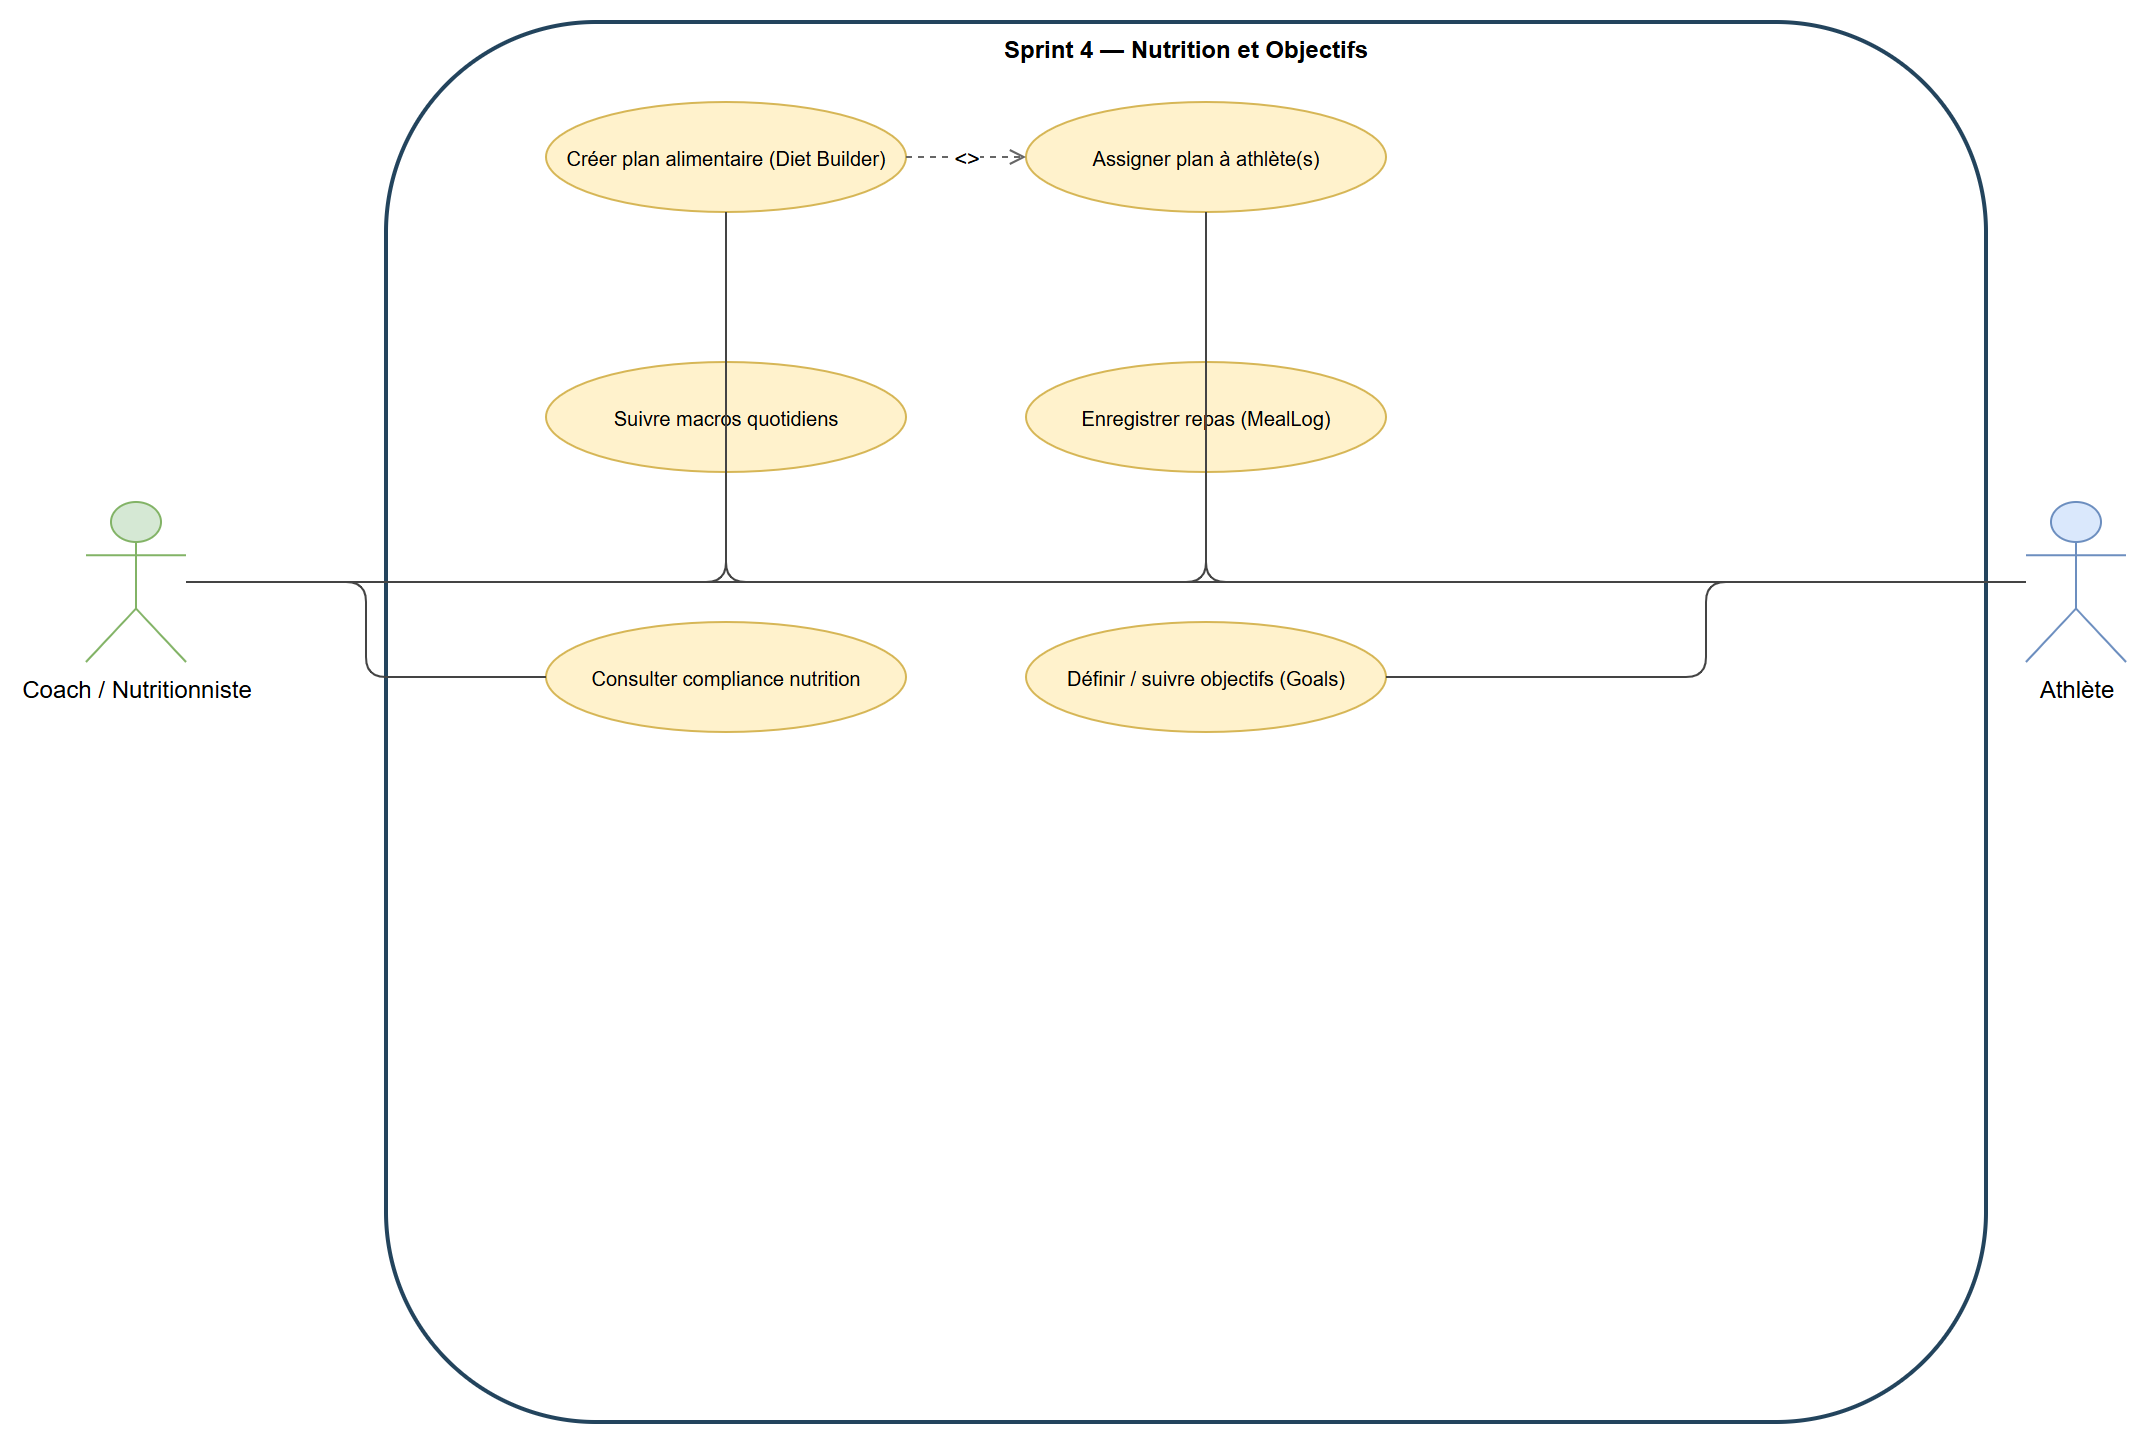
\includegraphics[width=0.85\textwidth]{diagrams/use case sprint 4.png}
\caption{Diagramme des cas d'utilisation - Sprint 4}
\end{figure}

\subsection{Diagramme de classes (Sprint 4)}
Pour supporter l'historique temporel des mensurations sans surcharger la table utilisateur principale, nous avons introduit l'entité \texttt{BodyMetric}. Chaque enregistrement est lié à un utilisateur par une relation de type "Plusieurs-à-Un" (Many-to-One), permettant de stocker une infinité de points de mesure dans le temps.

\begin{figure}[H]
\centering
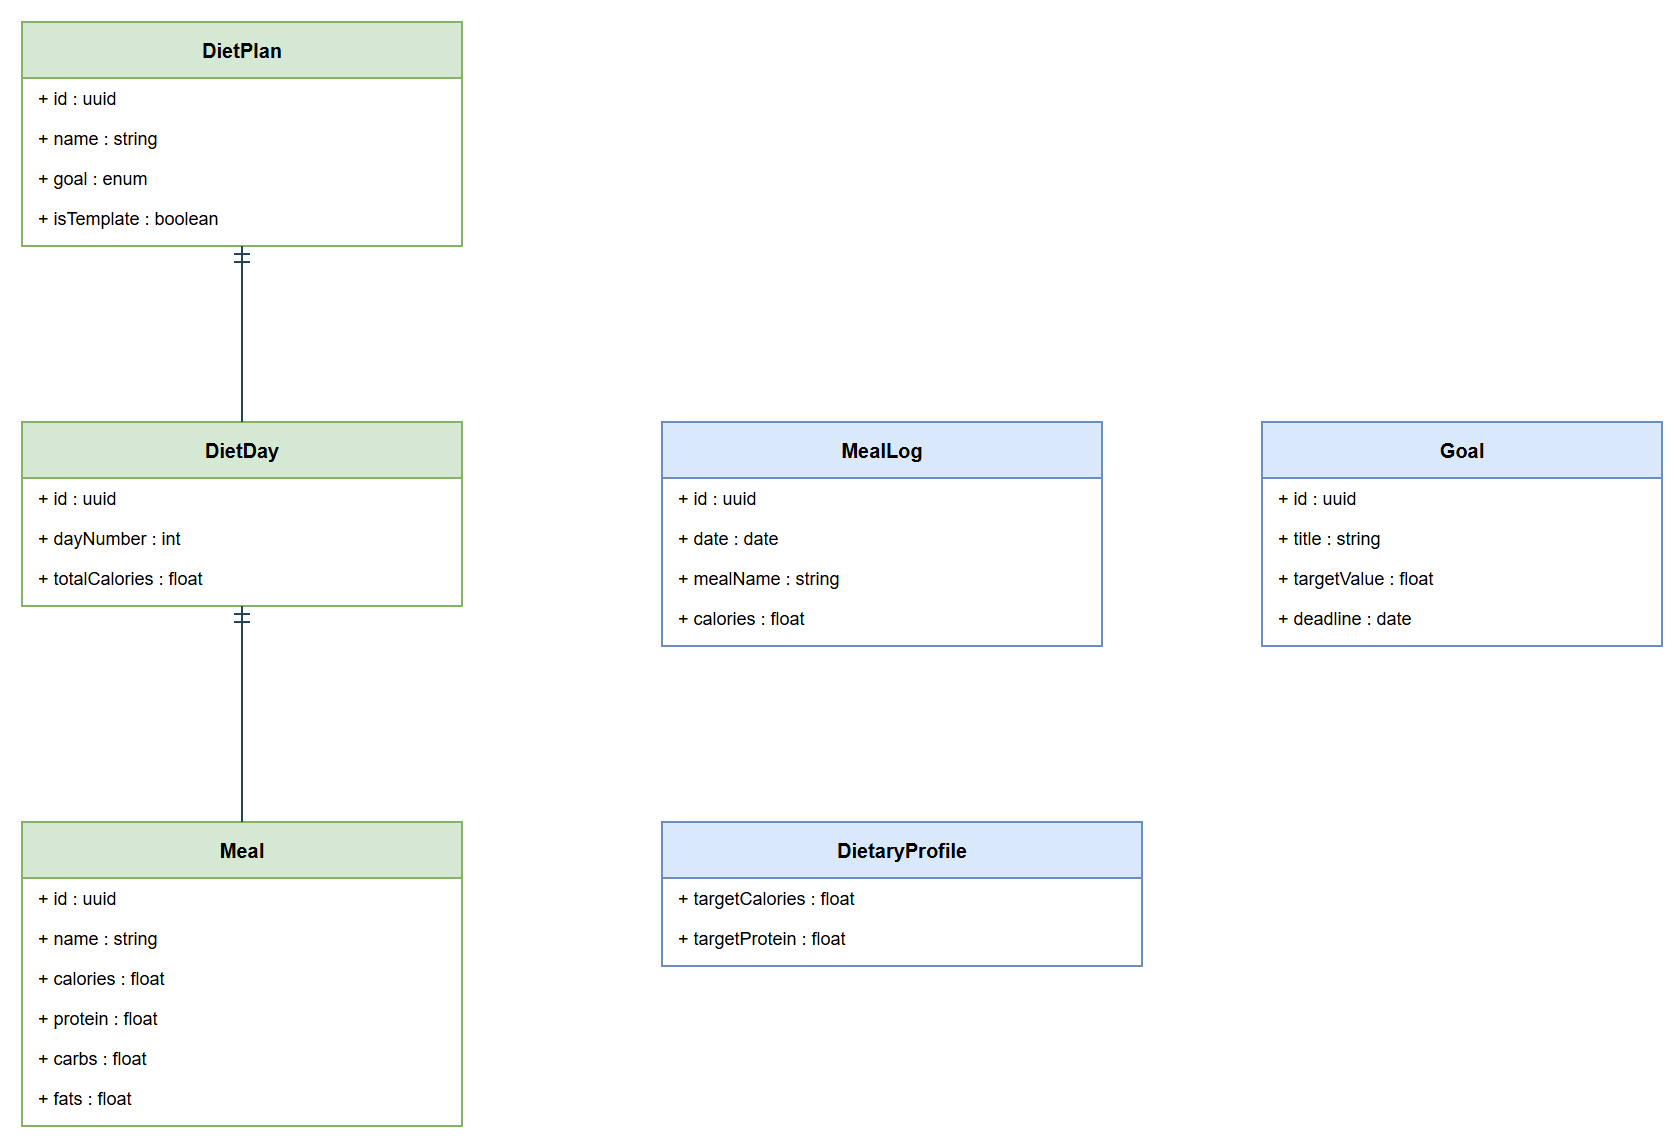
\includegraphics[width=0.9\textwidth]{diagrams/classe sprint 4.png}
\caption{Diagramme de classes étendu - Sprint 4}
\end{figure}

\subsection{Spécification du flux de synchronisation IoT}
La synchronisation des objets connectés repose sur un flux asynchrone sécurisé :
\begin{enumerate}
    \item L'application Flutter demande l'autorisation explicite à l'utilisateur de lire les types de données souhaités (Pas, Sommeil, Fréquence cardiaque).
    \item Le système d'exploitation (iOS ou Android) affiche la boîte de dialogue système de sécurité.
    \item En cas d'accord, le client Flutter interroge l'API locale du smartphone.
    \item Les données récupérées sont agrégées par jour, puis transmises en lot (Bulk Upload) vers le serveur Node.js.
\end{enumerate}

\section{Réalisation technique : La Synchronisation Objets Connectés}
\subsection{Intégration Flutter avec les API Health (Google/Apple)}
Pour unifier le développement sur iOS et Android, nous avons configuré le package Flutter \texttt{health} qui sert de couche d'abstraction commune au-dessus de Google Fit et Apple HealthKit. Le code Dart suivant illustre la méthode permettant de demander les autorisations et de récupérer le volume de pas quotidiens de la semaine passée.

\begin{lstlisting}[language=dart, caption={Service de synchronisation d'activité physique en Flutter}, label={lst:flutter_health}]
import 'package:health/health.dart';

class HealthSyncService {
  final HealthFactory health = HealthFactory();

  Future<int> fetchTodaySteps() async {
    // Definir les types de donnees a collecter
    List<HealthDataType> types = [HealthDataType.STEPS];
    
    // Demander l'autorisation d'acces a l'utilisateur
    bool requested = await health.requestAuthorization(types);
    
    if (requested) {
      var now = DateTime.now();
      var midnight = DateTime(now.year, now.month, now.day);
      
      // Recuperer les donnees du capteur pour la journee courante
      List<HealthDataPoint> healthData = await health.getHealthDataFromTypes(
        midnight, now, types
      );
      
      int totalSteps = 0;
      for (var x in healthData) {
        totalSteps += int.parse(x.value.toString());
      }
      return totalSteps;
    }
    throw Exception("Permission d'acces aux donnees de sante refusee");
  }
}
\end{lstlisting}

\subsection{Modélisation de l'historique sur le Backend (Node.js/TypeORM)}
Côté serveur, nous avons créé l'entité \texttt{BodyMetric} pour archiver les données anthropométriques complexes. Les données sont validées en amont avec Zod pour garantir l'absence de valeurs aberrantes (ex: poids négatif).

\begin{lstlisting}[language=TypeScript, caption={Entité TypeORM pour le suivi anthropométrique}, label={lst:body_metric_entity}]
import { Entity, PrimaryGeneratedColumn, Column, ManyToOne, CreateDateColumn } from 'typeorm';
import { User } from './User';

@Entity('body_metrics')
export class BodyMetric {
    @PrimaryGeneratedColumn('uuid')
    id: string;

    @Column({ type: 'float' })
    weight: number; // en kg

    @Column({ type: 'float', nullable: true })
    fatPercentage: number; // en %

    @Column({ type: 'float', nullable: true })
    muscleMass: number; // en kg

    @Column({ type: 'float', nullable: true })
    waistCircumference: number; // en cm (mensuration taille)

    @Column({ type: 'float', nullable: true })
    chestCircumference: number; // en cm (mensuration poitrine)

    @ManyToOne(() => User, user => user.id, { onDelete: 'CASCADE' })
    user: User;

    @CreateDateColumn()
    measuredAt: Date;
}
\end{lstlisting}

Les routes exposées permettent au coach de requérir ces listes chronologiques sous forme de tableaux ordonnés par date. Ces données sont ensuite injectées dans la vue Angular sous forme de graphiques de tendances à l'aide de \texttt{Chart.js}.

\section{Conclusion}
L'intégration accomplie au cours du Sprint 4 marque un tournant majeur pour CoachingApp. En connectant l'écosystème mobile aux objets connectés et en structurant l'historique des données morphologiques, nous offrons aux coachs des indicateurs de suivi d'une précision scientifique inédite. L'athlète n'a plus à saisir manuellement ses statistiques d'activité, ce qui accroît considérablement la rétention d'utilisation. Forts de cette base de données physiologiques, nous pouvons aborder le cinquième sprint axé sur la collaboration directe en temps réel par visioconférence et la prise de rendez-vous en ligne.
